\chapter{Systems Evaluation}
\label{chptr:evaluation}

As already stated, the actual system will be located within the context of the ~\gls*{ETCS}, more precisely within \abr{ETCS} level one.
Information in \gls*{ETCS} can be quite diverse in terms of type, size, durability, actualization frequency, and priority.
For example, a train's position is a periodically and frequently updated type of information, while a \gls*{MA} is valid for a longer time and may be updated unfrequently.
There is also a difference in whether the information is kept as a state of the system, used as a message within the system, or if it is provided as system input, where system state is derived from.

\section{Events and States in \abr{DDS}}
In this section, an overview about different information types and possibilities for their representation in \gls*{DDS} topics is provided.

\begin{table}[h!]
	\begin{center}
		\caption{\Gls*{QOS} policies for volatile and enduring states in a \gls*{DDS} system. For an enduring state, data changes slow and unperiodically. In volatile states, data changes frequently and periodically.}
		\label{tab:stateQOS}
		\begin{tabularx}{\textwidth}{|X|X|X|X|}
			\hline
			\textbf{QoS policy} & \textbf{Setting for volatile state} & \textbf{Setting for enduring state} & \textbf{Description}\\
			\hline \hline
			Deadline & Depends on actual implementation & Not required & For volatile state, the deadline should match the period in which the data updates. \\
			\hline
			DestinationOrder & SourceTimestamp & SourceTimestamp & Using the source timestamp as ordering guarantees that always the most recent data is stored. \\
			\hline
			Durability & Volatile & Transient or Persistent & The more frequent the state changes, the less critical it is for late joining subscribers to see previouly published data. \\
			\hline
			History & KeepLast(1) & KeepLast(1) & Most of the time, only the last state matters. \\
			\hline
			LatencyBudget & Depends on actual implementation & Not required & The maximum acceptable delay for sending the data should be choosen so that deadlines are not missed. \\
			\hline
			Reliability & BestEffort & Reliable & For rapidly and periodically changing state, it is ok if some data gets lost. For enduring state however, data has to be transferred reliably. \\
			\hline
			WriterDataLifecycle & Not required & autodispose\_unregistered\_instances = False & Even if data instances are unregistered, the actual data should not be disposed on enduring state topics. \\
			\hline
		\end{tabularx}
	\end{center}
\end{table}

A train's speed or position data, as well as currently valid \abrpl{MA}, are examples for the system's state.
A state could contain perodically changing data, or irregular changing data, respectively.
A state whose data changes periodically is called a volatile state, while a state whose data changes slow and irregular is called an enduring state.
Possible \gls*{QOS} settings for volatile and enduring states are presented in~\autoref{tab:stateQOS}.

\begin{table}[h!]
	\begin{center}
		\caption{\Gls*{QOS} policies for events in a \gls*{DDS} system.}
		\label{tab:eventQOS}
		\begin{tabularx}{\textwidth}{|X|X|X|}
			\hline
			\textbf{QoS policy} & \textbf{Setting} & \textbf{Description}\\
			\hline \hline
			Deadline & Depends on actual implementation & For periodically updating events, a deadline can be specified to detect when events are missing in a period. \\
			\hline
			DestinationOrder & SourceTimestamp & The event samples should be ordered based on the time they got produced. \\
			\hline
			Durability & Depends on actual implementation & It might be appropriate to let late joining DataReaders process the events. \\
			\hline
			History & KeepAll & All events shall eventually be send and processed. Therefore, the event samples should be stored on both the sender and the receiver side.  \\
			\hline
			Lifespan & Depends on actual implementation & A event may be only valid for a specific period of time. This timespan can be specified by assigning a ifespan to a DataWriter. \\
			\hline
			Reliability & Reliable & The middleware will attempt to deliver all event data samples and actively checks if the receivers got them. In case the samples got lost, they are re-transmitted. \\
			\hline
			ResourceLimits & Depends on actual implementation & It might be appropriate to specify an upper bound for resouces to be allocated. Especially with History set to KeepAll. \\
			\hline
			WriterDataLifecycle & autodispose\_unregistered\-\_instances = False & Unregistered data instances should not be disposed because the events are required to be eventually processed. \\
			\hline
		\end{tabularx}
	\end{center}
\end{table}

Certain circumstances, such as the availablity of track-side information or the exceeding of speed limits, need to be processed as soon as possible.
Such data is typically expressed as events and can be represented using event topics.
\autoref{tab:eventQOS} provides an overview about \gls*{QOS}-policy settings for event topics.
The presented combination of \abr{QOS}-settings ensures that events are eventually processed in the order they were issued and that no event is omitted.
While some settings are universal for event topics, some others need to be evaluated with regards to an actual system implementation and consequential requirements.

%\subsection{High-Level Risk Analysis}

\section{System Design and Comparison}
The different redundancy techniques, as proposed by Johnson Barry, are applicable for different use-cases~\cite{BarryFaultToleranceAnalysis}.
In this section, different redundancy techniques are selected, combined and evaluated based on following criteria:

\begin{itemize}
\item \textbf{Safety:} How likely is the system to reliable detect an error and transition the system into a safe state.
\item \textbf{Implementability using \gls*{DDS}:} How easy is it to implement the redundant architecture using \abr{DCPS} concepts.
\end{itemize}

In order to evaluate the redundant system's safety, it is mathematically evaluated using Marcov Chains, as described in~\autoref{sec:safetyEvaluation}.
For investigating the technique's implementability with \gls*{DDS}, the required functionalities and \gls*{QOS} policies for setting up the architecture, are proposed and examined.
\\

%------DDS-------
All computing systems have in common, that they receive an input and produce an output.
In the exemplary case that is considered in this thesis, the system's input can be trasmitted using \abr{DDS} topics.
Such an \texttt{Input}-topic should be defined as an event topic to make sure that every replica receives and eventually processes the inputs.
Because inputs occur asynchronously, the deadline \gls*{QOS} is not applicable for the \texttt{Input} event topic.
For real-time applications, as examined in this work, an output is expected to be delivered by the sytem withing a maximal timespan of $\Delta t$ after the system received an input.
Therefore, the input topic's \texttt{Durability} should be set to volatile and the \texttt{Lifespan}-policy should be set to at least $\Delta t$ plus a network latency.
The input's \texttt{ResourceLimit} depends on the frequency the input is expected to be delivered and can be set to one when the input's frequency is higher than $\Delta t$.
\\

The components in a redundant system are required to communicate with one another because at the end, the entire system needs to present a single result.
In the course of this thesis, all communication in the system will be implemented using \abr{DDS} event topics because it should be ensured that, given a sufficient network, no information is lost in the system.
Thus, the communication topic's \gls*{QOS}-settings can be the same as for the input topic.
However, the \texttt{Lifespan}-policy needs further specification, because the replicas are independent and messages might be delayed due to network latency.
After a specific time, however, certain message might not be valid anymore.
An example for this could be message concerning a \abr{MA} that has been expired by the time the delayed information was received.
A component's message might therefore require a certain \texttt{Lifespan} that depends on the actual message.
\\

The minimal communication overhead required in a redundant system is between the replicas and the voter.
As described earlier, voters can either be implemented in software, or in hardware.
This does not hold for redundant systems where \gls*{DDS} is used for the communication between the replicas and the voter because the voter always requires a software part that implements the \gls*{DCPS} standard.

One of the most commonly used redundancy techniques is \gls*{TMR}~\cite{FaultToleranceViaNMR}, which will therefore constitute the foundation for further system investigations.

\subsection{Triple Modular Redundancy}
\Gls*{TMR} was already briefly discussed in~\autoref{sec:redundancyPatterns} and is depicted in~\autoref{fig:Classical2OO3}.
The reliability and safety characteristics of \gls*{TMR} have been studied in depth, for example by Arifeen \etal~\cite{ArifeenFaultTolerantTMR}.
Their findings show that the reliability of \gls*{TMR}-systems ($R_{TMR}(t)$) is given by the sum of the probability of all three components functioning and two components functioning.

\begin{equation}
R_{TMR}(t) = 3e^{-2 \lambda t} - 2e^{-3 \lambda t}
\end{equation}

This equation only holds for homogeneous redundancy and when the components are independent.
While the independence is is a precondition for the exponential failure law, a diverse system can be described in the same way by using a distinct $\lambda$ for each component.
\\

The first four fault classes from~\autoref{sec:techniquesSafetyReliability} for at most one failing replica can be tolerated by a triple modular system.
For example, if one replica produces a wrong result, the voter still receives two correct results and can mask the wrong result using a majority voting.
However, if two or more replicas produce the same, but wrong result, the voter erroneously accepts the wrong result as the majority.
On the other hand, if two or more replicas fail to produce on output within a certain time span, the voter can detect this as a deadline violation and can transfer the system into a safe state, e.g. by stopping the train.
Therefore, only \textbf{F1}, \textbf{F2}, and \textbf{F3} can be detected when more than one replica is affected in \abr{TMR}.

This is different, when a component's wrong result is based on a corrupt internal consistency and component checking mechanisms are applied.
In this case, the faulty components can be determined and \textbf{F4} can also be covered by excluding the faulty components from the voting so that the system remains safe.

Nevertheless, a failed voter can render the entire system unsafe, because it marks a single point of failure in \abr{TMR}.
Therefore, the entire system's reliability and safety cannot be higher than the voter's reliability and safety~\cite{ArifeenFaultTolerantTMR}.
The same holds true for the applied communication channel, when only a single one is used.

Another problem arises when the frequency in which inputs occur is higher than the time that the system needs to produce an output.
In such a case, an output might be already outdated even before it is being produced.
\\

Recapped, \abr{TMR} suffers four major challenges, which being

\newcommand{\ChallengeWR}{\textbf{Multiple Wrong Results}\xspace}
\newcommand{\ChallengeVoter}{\textbf{Single Voter}\xspace}
\newcommand{\ChallengeComm}{\textbf{Single Communication Channel}\xspace}
\newcommand{\ChallengeThrough}{\textbf{Throughput Cap}\xspace}
\begin{itemize}
\item \ChallengeWR When more than one replica produces a wrong result, \abr{TMR} is only safe if the wrong result happened because the affected replica was not internally consistent and the replica's internal consistency is monitored.
\item \ChallengeVoter The voter marks a single point of failure.
\item \ChallengeComm The communication channel marks a single point of failure.
\item \ChallengeThrough A system's throughput time needs to be smaller than the frequency in which inputs occur.
\end{itemize}

\ChallengeComm can be solved with information redundancy techniques by introducing an additional communication channel.
Again, diverse redundancy can further improve the safety and reliability because it excludes errors that are specific to a certain communication technology.
For example, one communication channel could use Ethernet as and another could be via CAN-bus.
\\

In order to solve \ChallengeVoter and prevent the voter from being a single point of failure, redundancy can be introduced for the voters as well.
However, this introduces new challenges such as the possibility of a split brain, where multiple voters are active and can manipulate the output at the same time.
A solution for this are discussed later in~\autoref{subsec:consensusArchitecture}.
\\

In order to achieve \ChallengeWR, each replica's internal consistency needs to be monitored.
This could be done in two ways, either each replica monitors itself and reports its internal consistency via periodic heartbeat messages, or each replica is monitored by another component in the system.
When a replica monitors itself, it is also responsible to exclude itself from the voting process when its internal consistency is faulty.
Further, the affected replicy needs to notify other components, e.g. the voter, about this fact.
The notification should be done via a \abr{DDS} event topic to ensure that the other components are informed.
Another way would be to store information about a replica's internal consistency in an enduring \abr{DDS} state, so that it is retrievable by each subscriber at any time.
It depends on the actual implementation, which method is more applicable.
\\

Another way to allow more replicas to fail and produce the same wrong result would be to add more replicas
It can be shown via induction, that adding more replicas increases a system's reliability.

\paragraph{Proof by induction}
Let $M$ be contant and $M \leq N$, let $R_{c}$ the reliability of the system's components.

\subparagraph{Basis}
\begin{align*}
&Let N = 1 \Rightarrow M = 1.\\
&R_{1oo1} = {1 \choose 1} * R_{c}^1 * (1 - R_{c})^0 = R_{c}
\end{align*}

\subparagraph{Hypothesis}
\begin{center}
$R_{MooN}$ describes the reliability for a M-out-of-N-system and a components reliability $R_{c}$ can only be positive.
\end{center}

\subparagraph{Inductive}
\begin{align*}
R_{MooN+1} &= \sum_{i=M}^{N+1} {N + 1 \choose i} * R_{c}^i * (1 - R_c)^{N + 1 - i}\\
&= \sum_{i=M}^{N} {N \choose i} * R_{c}^i * (1 - R_c)^{N - i} + {N+1 \choose N+1} * R_c^{N+1} * (1 - R_c)^{N+1 - N+1}\\
&= R_{MooN} + R_c^{N+1} \\
&\Rightarrow R{MooN} \leq R_{MooN+1} \quad \square
\end{align*}

\subsection{\Gls*{TMR} with spares}
\begin{figure}[!hb]
	\centering
	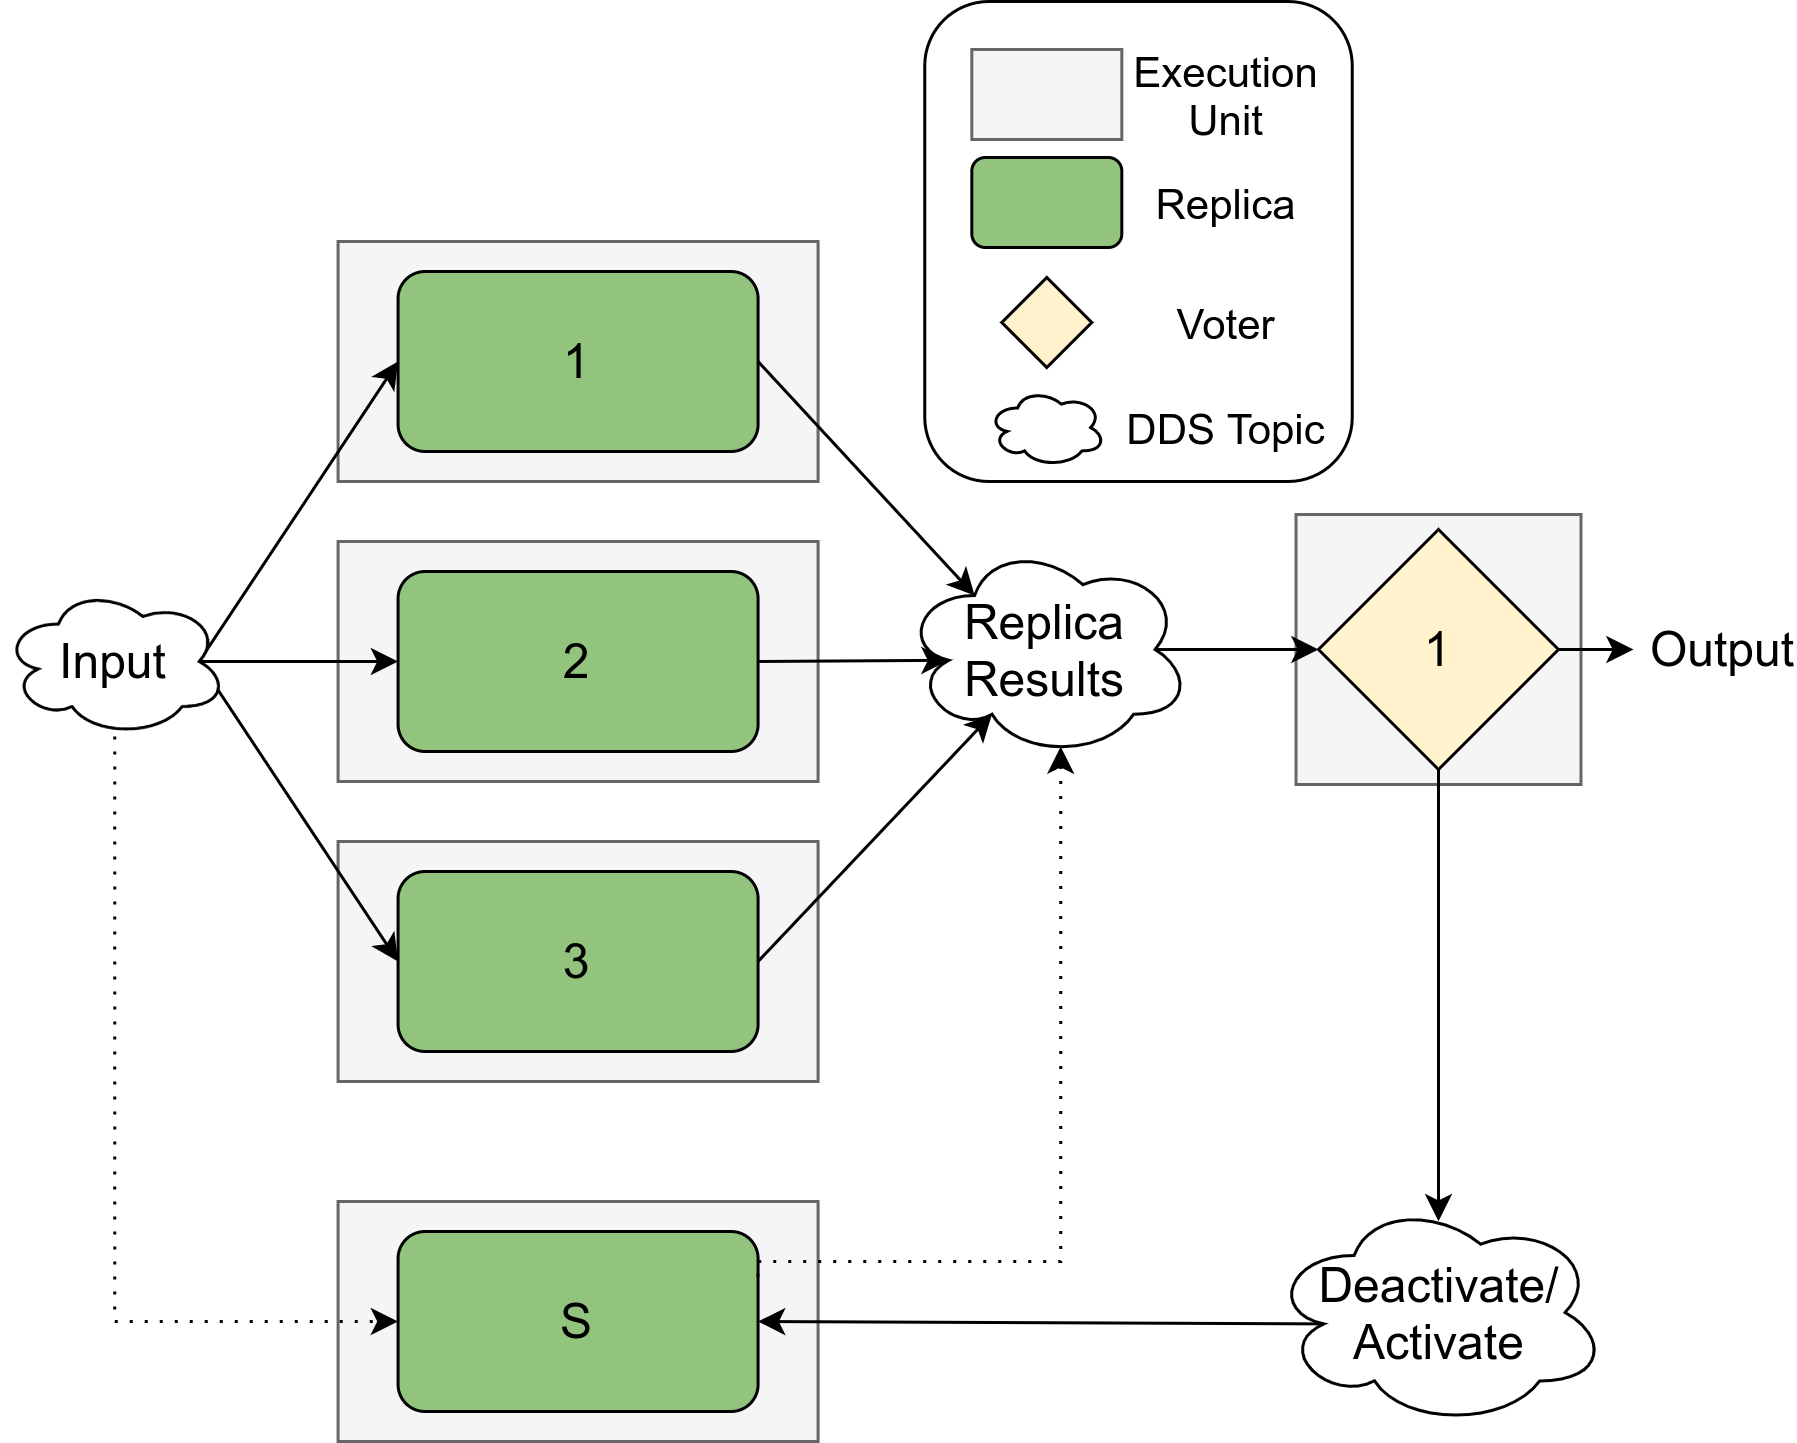
\includegraphics[width=0.75\linewidth]{images/TMRWithSparesDDS}
	\caption{A hot standby can be implemented using \abr{DDS} event topics. In this case, the voter is responsible for detecting when a replica crashed and activates a spare component in this case by sending a corresponding event.}
	\label{fig:TMRWithSparesDDS}
\end{figure}

Instead of adding more replicas in a passive hardware redundancy way, they can also be added as spares in an active hardware redundancy approach.
However, this also increases costs and communication overhead.

Standby redundancy is a way for redundant systems to repair themselves in case of failures by adding spare replicas, that can replace faulty replicas.
Therefore, the system relies on error detection methods.
For the reliability of \abr{TMR} with a spare component holds, provided that the system can reliable detect and repair any error and the replicas are homogeneous and independent:

\begin{equation}
R_{TMR\_S}(t) = 2 * {3 \choose 3} e^{-\lambda t} + {3 \choose 2} e^{-\lambda t}
 = 3e^{-2 \lambda t} - e^{-3 \lambda t}
\end{equation}

One way of implementing \abr{TMR} with a spare using \abr{DDS} is depicted in~\autoref{fig:TMRWithSparesDDS}.
The input, as well as the replica's results and an activate event are modelled as \abr{DDS} event topics.
In an exemplary case, where one replica crashes, the voter would receive only two replica results and thereupon sends an activate event via the corresponding topic.
When the spare replica (S) receives the activate event, is subscribes the the \texttt{Input} topic and registers to the \texttt{Replica Results} topic to publish data to it.
In case the failed replica comes back to life and the voter recognizes this, the voter can reject the result from (S) and send a deactivate event.
Thereafter, the spare replica ends its subscription to the input topic and stops publishing results.
A precondition for this approach is, that a replica's result can be unambiguously assigned to a replica, for example by using IDs or by using an individual result topic for each replica. 
\\

Although \abr{TMR} with spares improves the replicated system's reliability and addresses \ChallengeWR, the voter remains a single point of failure (\ChallengeVoter) and the system's throughput has not changed (\ChallengeThrough).

\subsection{Pipelined \abr{TMR}}
\begin{figure}[!hb]
	\centering
	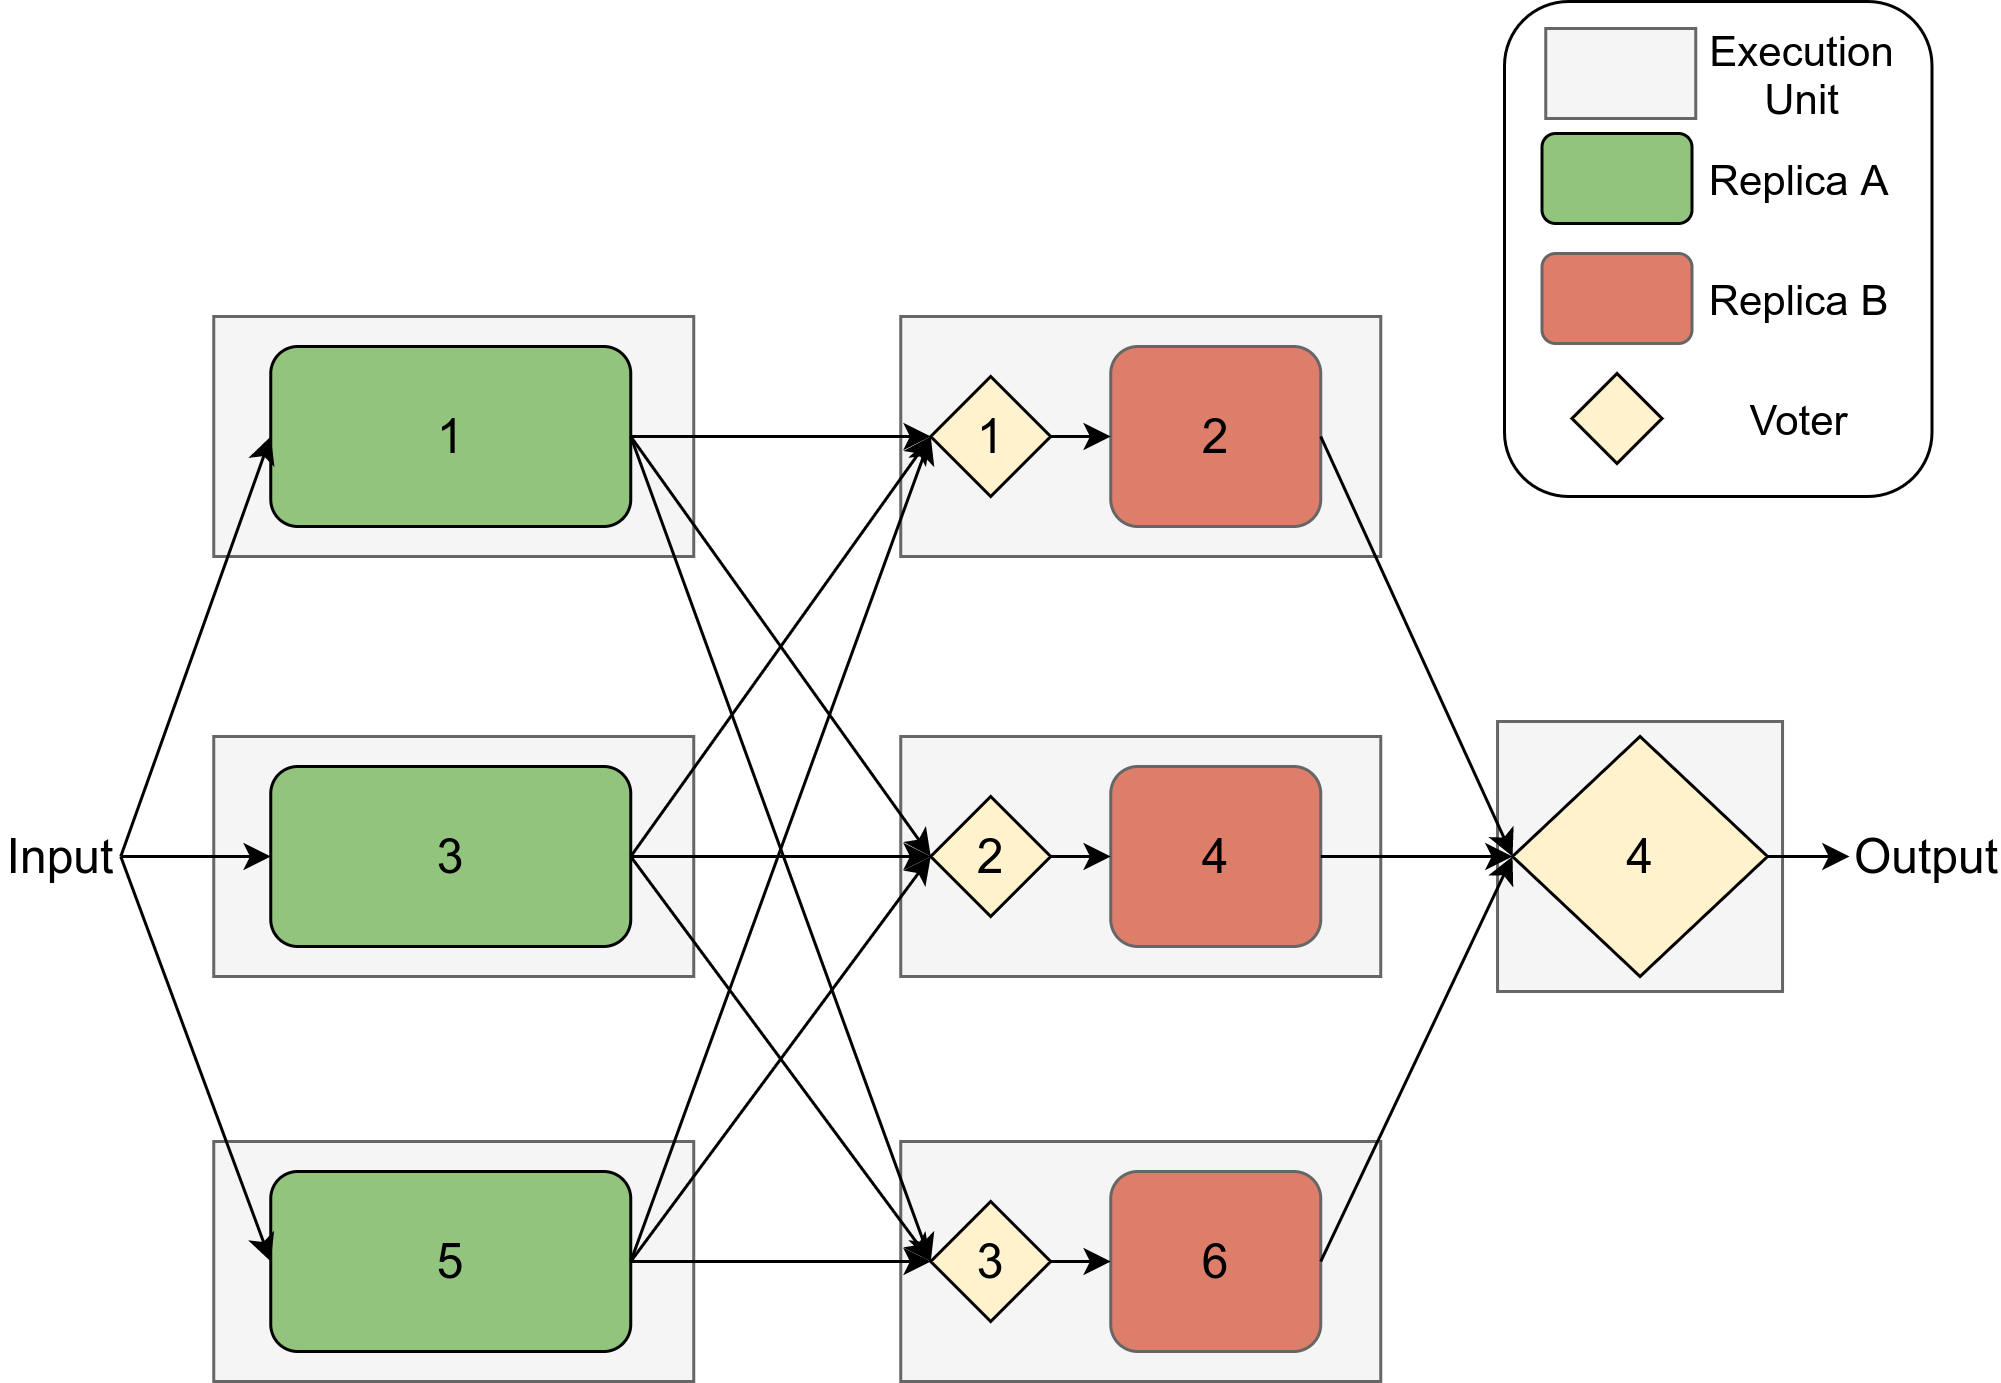
\includegraphics[width=0.75\linewidth]{images/InterconnectedVoterPipeline}
	\caption{Two interconnected pipeline streams with on-component intermediate voting can improve throughput. However, it also increased the system's cost, complexity and communication overhead.}
	\label{fig:PipelineIntermediateVoters}
\end{figure}

In order to improve a system's throughput, an often applied technique is pipelined computation~\cite{TanenbaumSteen07}.
In a pipelined approach, intermediate voting should be used to reduce the effect of wrong intermediat results.
It is further possible that components function as both a voter and a data processing replica.
A paradigmatic redundant and pipelined system with intermediate voting on replicas is depicted in~\autoref{fig:PipelineIntermediateVoters}, where voters (1), (2), and (3) each perform a majority voting based on the results from replicas (1), (3), and (5).
Based on the voted intermediate results, replicas (2), (4), and (6) can perform their dedicated calculations and produce an individual output which is later reduced by voter (4).
Thereby, any failure from replicas (1), (3), or (5) can be masked before they are even handled to the final voter (4).
However, this approach is still a two-out-of-three approach and therefore has the same challenges that \abr{TMR} has.
Further, the pipelined approach's reliability can be calculated in the same way as for \abr{TMR}, because in a worst case, two replicas of type A or type B could fail.
\\

Although the pipelined approach enhances the system's thoughput, it also enhances the computation and communication overhead, as well as the system's cost.
Thus, a tradeoff needs to be made between the added throughput and the additional computation and communication overhead, as well as the increased cost for the system.

Again, the reliability evaluation can only be made without evaluating the voter - in the pipelined version voter (4) - which remains a single point of failure.
As proposed previously, this can be solved by adding redundancy for the voter as well, like for voters (1), (2), and (3) in~\autoref{fig:PipelineIntermediateVoters}.
In such a system, it needs to be ensured that only a single voter is in charge of controlling the system's final output.
This can be achieved by applying a consensus algorithm.
%When letting a single instance, for example a designated replica, decide about the availability and internal consistency of the voter, a new single point of failure would be introduced in the form of this replica and nothing would have been achieved.
%When each replica by itself decides about the voter's availability, a splic brain situation could arise because of network latencies.
%A way to prevent both of these problems is though a consensus algorithm.

\subsection{Consensus-inspired Architectures}
\label{subsec:consensusArchitecture}
\begin{figure}[!hb]
	\centering
	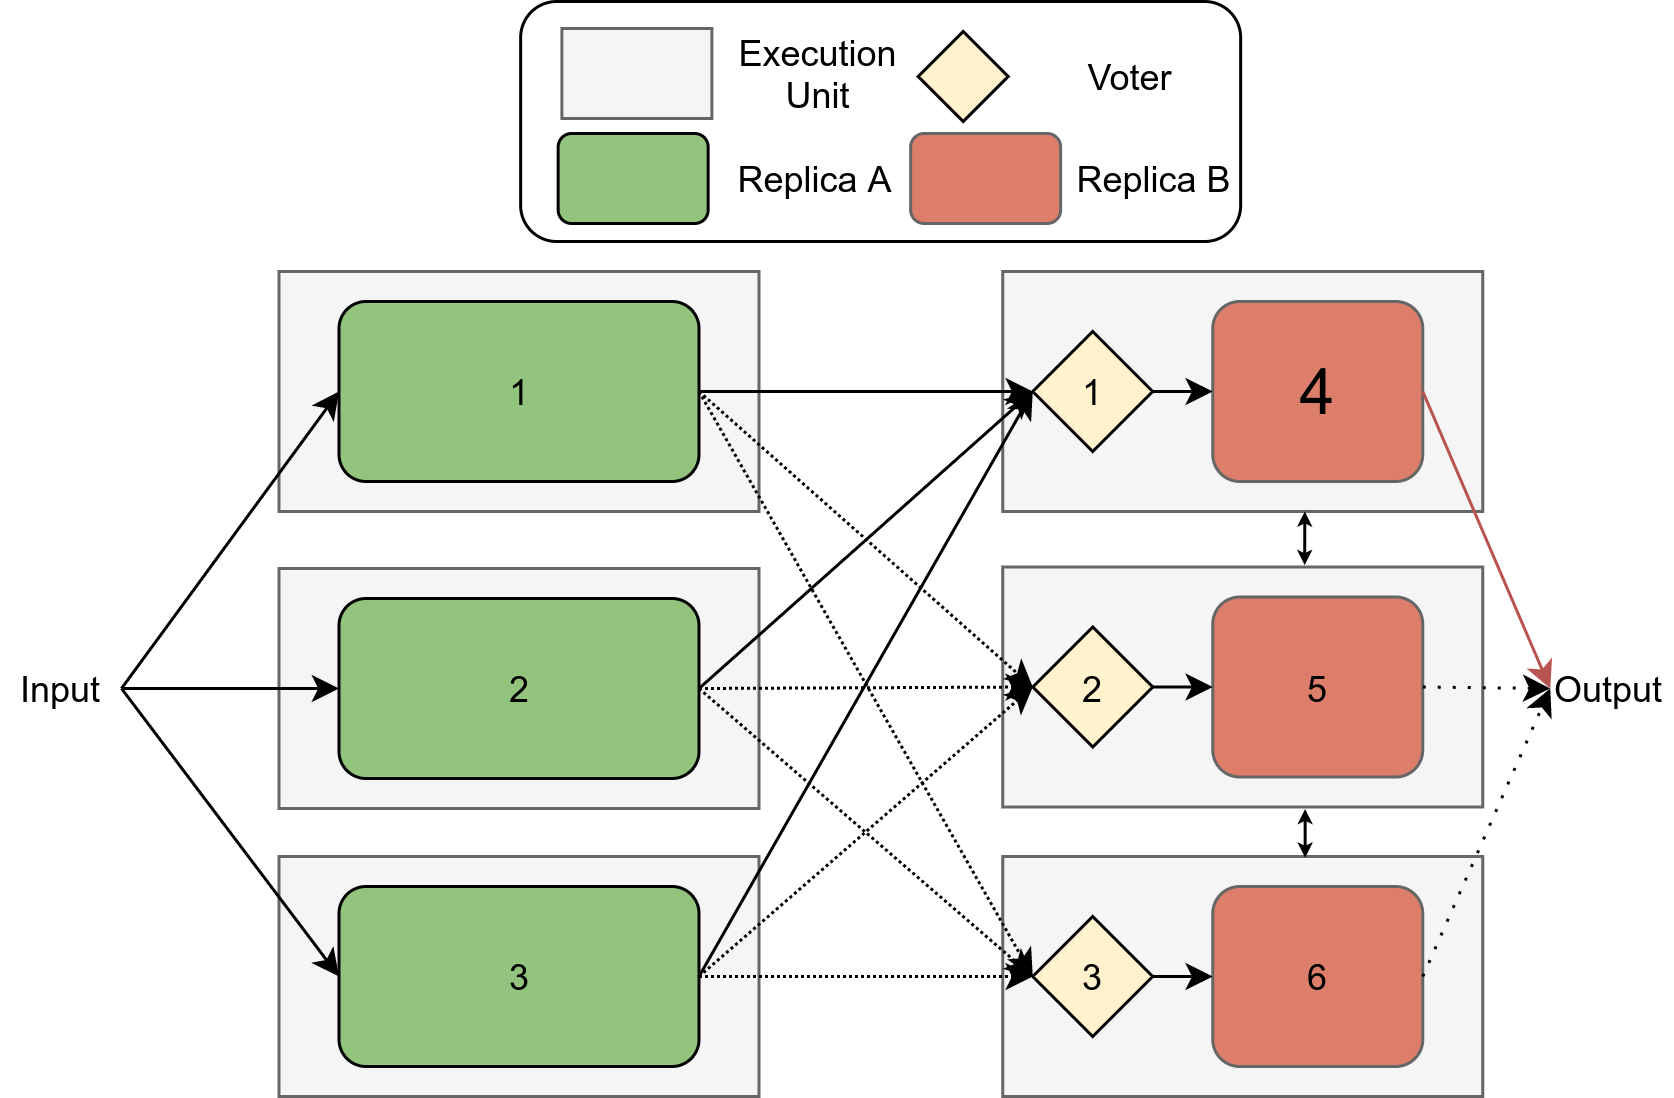
\includegraphics[width=0.75\linewidth]{images/ThreeComponentConsensus}
	\caption{An alternative to a voter can be a consensus algorithm. In this example, which follows basic ideas from \texttt{Raft}, replica (4) with voter (1) took over the leader role.}
	\label{fig:ThreeRepConsensus}
\end{figure}

For a consensus, multiple components are involved in deciding about redundant information.
An exemplary consensus algorithm is \texttt{Raft}, which has been proposed by Ongaro and Ousterhout~\cite{RaftConsensusPaper}.
A component in \texttt{Raft} can take on one of three roles, namely \textit{leader}, \textit{follower}, or \textit{candidate}.
While a leader has the entire responsibility, followers wait for instructions from the leader and can become candidates in order to promote to become the new leader.
\texttt{Raft}'s leader election algorithm ensures that only one leader is active at a time and that the absence of a leader in the system is reliably detected.

An example of how the three roles from \texttt{Raft} are used is depicted in~\autoref{fig:ThreeRepConsensus}.
The replicas (1), (2), and (3) make up a \abr{TMR} system, while replicas (4), (5), and (6) together define a voter for the system.
The replicas (4), (5), and (6) toghether implement the consensus protocol and each provide a designated voter.
In the example of~\autoref{fig:ThreeRepConsensus}, replica (4) took over the leader role and thereby has complete control over the output, while (5) and (6) are followers.
\\

To sum it up, a redundant architecture using \abr{DDS} has been established step by step in this section.
\abr{TMR} was only able to mask a wrong result from one replica (\ChallengeWR) and suffered from the voter (\ChallengeVoter) and the communication channel (\ChallengeComm) being a single point of failure.
Further, the system's throughput might not be sufficient in \abr{TMR} (\ChallengeThrough).
\ChallengeComm could be solved by using redundant communication channels, following the idea of information redundancy.
In order to solve \ChallengeWR and to allow more replicas to fail without affecting the system's safety, more replicas could be added, either in an active, or in a passive redundant way.
An active approach for adding replicas was presented in the form of \abr{TMR} with spares.
To enhance a system's throughput, and thereby solve \ChallengeThrough, a pipelined \abr{TMR} was presented.
Finally, a possible solution for \ChallengeVoter was presented by replicating the voter and using concepts from consensus algorithms.